\chapter{Aufbau} \label{Aufbau}

%Kurze Erläuterung der Aufgabenstellung und der Messmethode, d.h. stichwortartige 
%Zusammenstellung von wesentlichen Definitionen, Formeln, etc. (keine Herleitungen, 
%keine seitenlange Darstellung von Lehrbuchwissen!). 

Der Versuchsaufbau ist in drei Aufbauten unterteilt. Der erste befasst sich mit der Charakteisierung des piezoelektrischen Wandler. Aufbau zwei und drei befassen sich
mit der Messung der Schallgeschwindigkeit bzw. die Messung der Laufzeit des Signals. Für die Aufbauten zwei und dre wird eine Benetzung der Kontaktflächen mit Ultraschallgel vorrausgesetzt. 

\section{Charakteisierung des Wandlers}

Zur Messung des Impedanzgangs des Wandlers wird der Piezo in Serie mit einem definierten Wiederstand geschalten.
Der Wiederstand dient dabei zur bestimmung des Stromes. Dabei wird die Spannung vor und nach dem Wiederstand (\SI{51}{\Omega}, \SI{2200}{\Omega}) abgegriffen. Daraus kann der Strom berechnet werden \( I = \frac{U}{R} \).
Die Auswertung erfolgt über eine Frewunezmodulation bei einer Amplitude von \(V_{pp} = 5 V \) über das LabVIEW-Programm impedance.vi \cite{laborpraktikum2022}.

%********************************************************
% Hier kommt noch ein Schaltplan rein
%********************************************************


\section{Messung der Schallgeschwindigkeit} \label{Aufbau_Schall}
Die Schallgeschwindigkeit wird über zwei Piezowandler und dem einem Probekörper gemessen. Ein Wandler wird dabei an einen Funktionsgenerator angeschlossen ( \( V_{pp} =5 V , f = 800 kHz , 1 MHz, 1.4 MHz \)), dieser dient als Sender der Schallwelle.
Der zweite Piezowandler wird gegenüber den ersten angebracht und an ein Oszilloskop angeschlossen. Der Aufbau ist in \autoref{img:Schall} ersichtlich. Die Einspannug dient dabei der Fixierung des Aufbaus.
Mittels der Laufzeit (Differenz aus Anregung und Empfang des ersten Messsignals) kann die Ausbreitungsgeschwindigkeit berechnet werden. \(c=\frac{\lambda}{T}\) Hierbei entsprich \(\lambda\) der Breite des Probelörpers und \(T\) der Laufzeit.
Der Versuch wird anschließend mit zwei Probekörpern in Serie wiederholt.


\begin{figure}[h]
    \begin{minipage}[b]{.50\linewidth} % [b] => Ausrichtung an \caption
       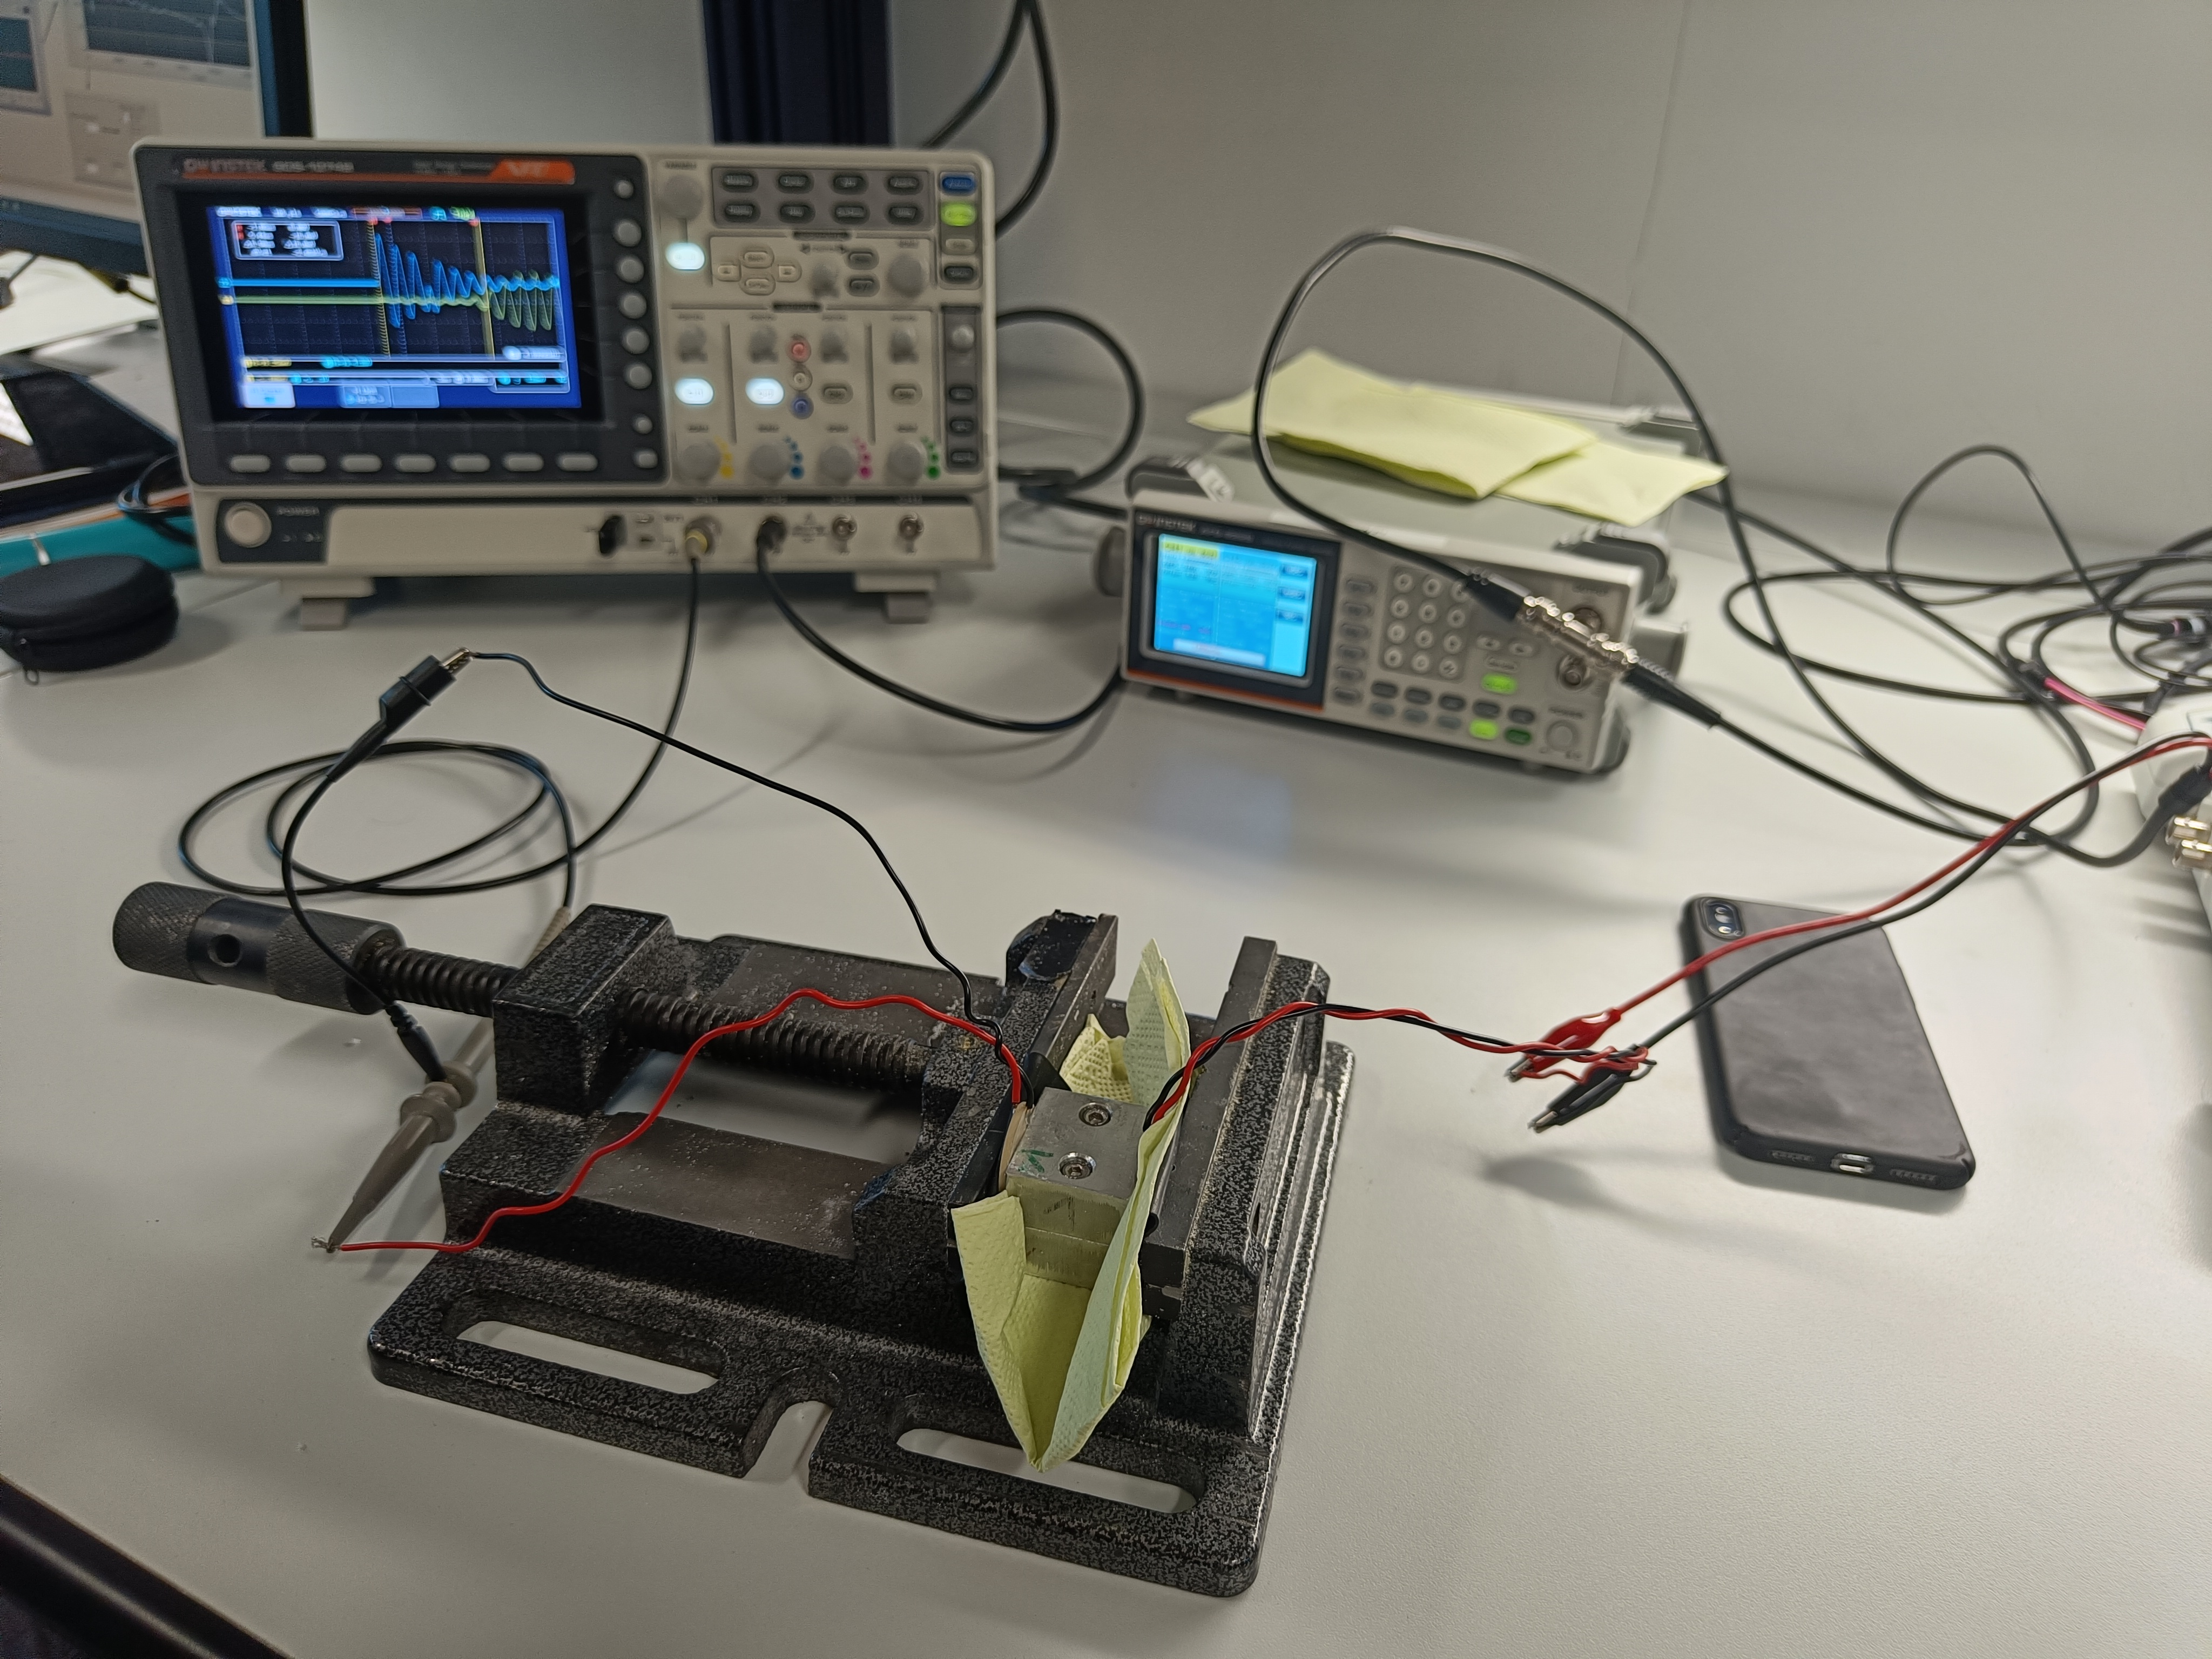
\includegraphics[width=\linewidth]{image/charakterisierung.jpg}
       \caption*{\textbf{a)}Messaufbau mit einem Probekörper}
    \end{minipage}
    \hspace{.01\linewidth}% Abstand zwischen Bilder
    \begin{minipage}[b]{.5\linewidth} % [b] => Ausrichtung an \caption
       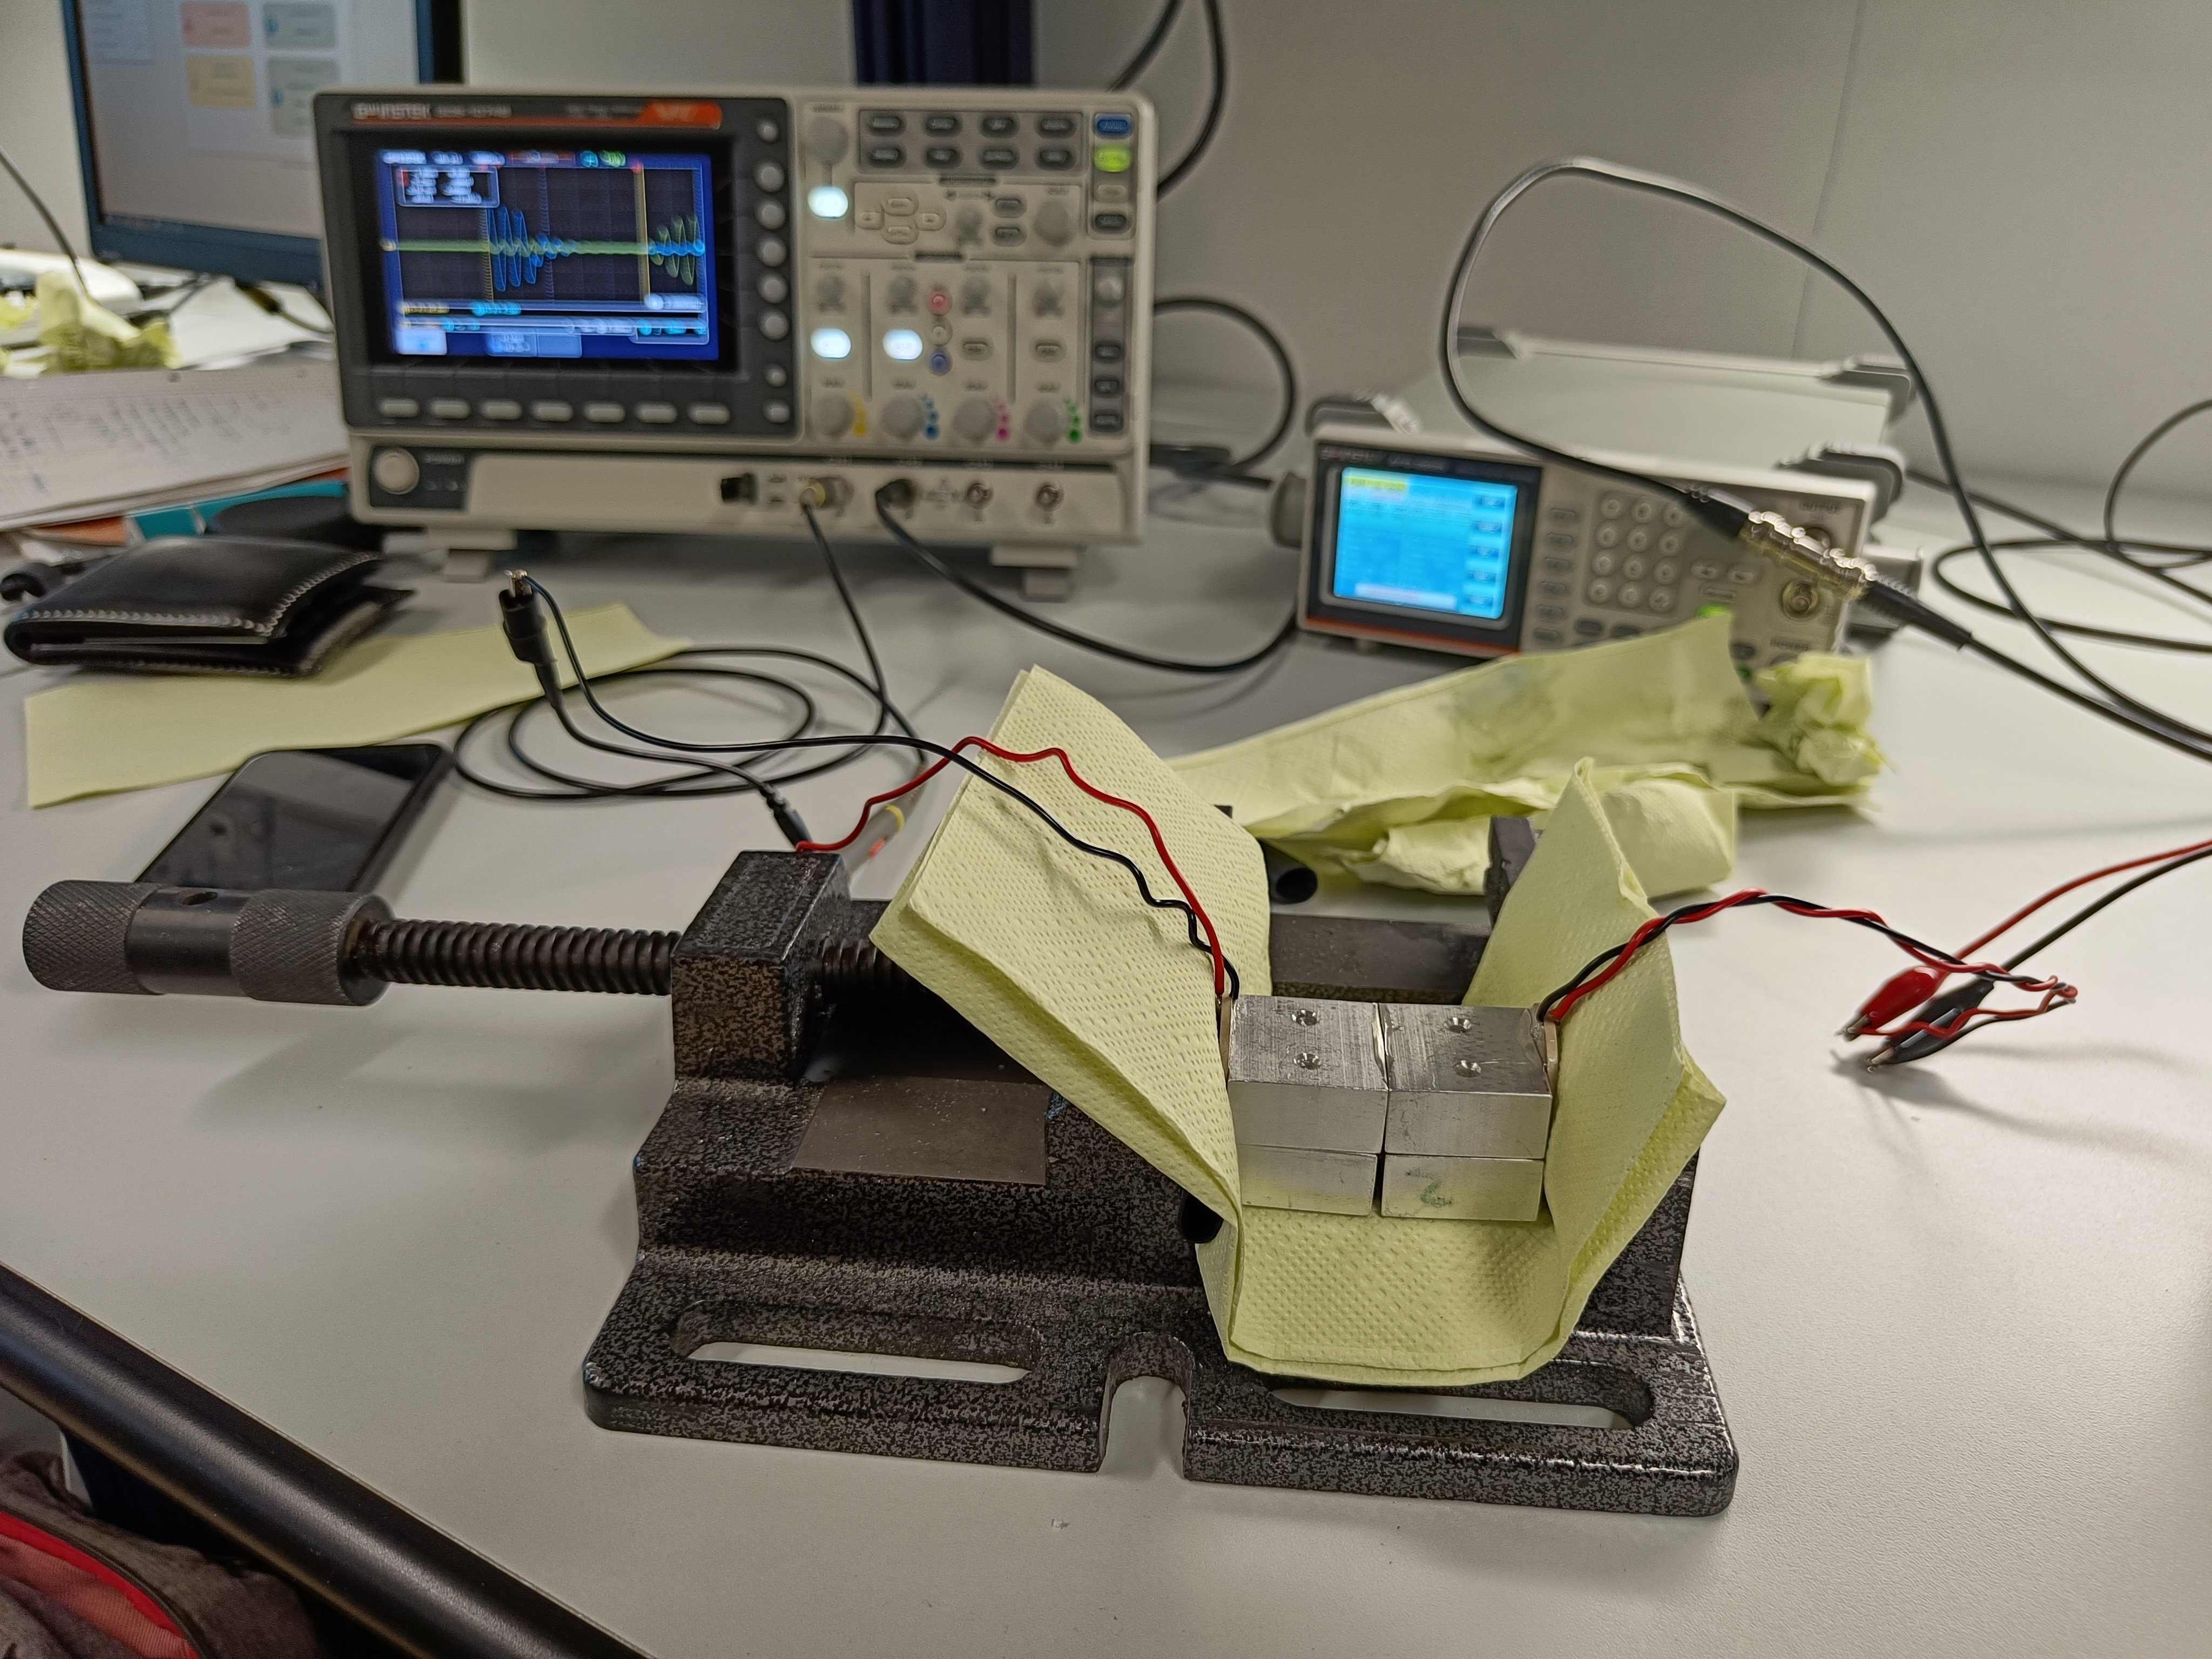
\includegraphics[width=\linewidth]{image/laufzeitmessung.jpg}
       \caption*{\textbf{b)} Messaufbau mit zwei Probekörpern}
    \end{minipage}
    \caption{Messaufbau Schallgeschwindigkeit zweiter Versuch}
    \label{img:Schall}
 \end{figure}





\section{Materialprüfung}

Für die Materialprüfung werden drei Probekörper vorbereitet. Einer besteht aus homogenen Material, einer beiinhaltet kleine Lufteinschlüsse und ein weiterer große Lufteinschlüsse.
Der Aufbau wird wie in \autoref{Aufbau_Schall} beschrieben durchgeführt. Der einzige unterschied ist, das die Probekörper paralell zur Schnnittfläche untersucht werden.



